\documentclass{article}

\usepackage{amsfonts}
\usepackage{amsmath}
\usepackage{amssymb}
\usepackage{amsthm}
\usepackage{caption}
\usepackage{color}
\usepackage{enumerate}
\usepackage{fancyhdr}
\usepackage[margin=1in]{geometry}
\usepackage{hyperref}
\usepackage{graphicx}
\usepackage{latexsym}
\usepackage{listings}
\usepackage{mathrsfs}
\usepackage[nottoc]{tocbibind}
\usepackage{setspace}
\usepackage{tikz}
\usepackage{tkz-graph}
\usepackage{url}

\providecommand{\all}{\ \forall \ }
\providecommand{\bs}{\backslash}
\providecommand{\e}{\varepsilon}
\providecommand{\E}{\ \exists \ }
\providecommand{\lm}[2]{\lim_{#1 \rightarrow #2}}
\providecommand{\m}[1]{\mathbb{#1}}
\providecommand{\mc}[1]{\mathcal{#1}}
\providecommand{\nv}{{}^{-1}}
\providecommand{\ov}[1]{\overline{#1}}
\providecommand{\p}{\newpage}
\providecommand{\q}{$\quad$ \newline}
\providecommand{\rt}{\rightarrow}
\providecommand{\Rt}{\Rightarrow}
\providecommand{\vc}[1]{\boldsymbol{#1}}
\providecommand{\wh}[1]{\widehat{#1}}

%\renewcommand\bibname{References}
%\renewcommand{\thesection}{Problem \arabic{section}}
%\renewcommand{\thesubsection}{Part \alph{subsection}}

\fancyhead{}
\fancyfoot{}
\fancyhead[R]{\thepage}
\fancyhead[C]{Landau}

\hypersetup{
    colorlinks,
    citecolor=black,
    filecolor=black,
    linkcolor=black,
    urlcolor=blue
}

\definecolor{dkgreen}{rgb}{0,0.6,0}
\definecolor{gray}{rgb}{0.5,0.5,0.5}
\definecolor{mauve}{rgb}{0.58,0,0.82}

\lstset{ 
  language=C,                % the language of the code
  numbers=left,
  numberfirstline=true,
  numbersep=5pt,                  % how far the line-numbers are from the code
  backgroundcolor=\color{white},      % choose the background color. You must add \usepackage{color}
  showspaces=false,               % show spaces adding particular underscores
  showstringspaces=false,         % underline spaces within strings
  showtabs=false,                 % show tabs within strings adding particular underscores
  frame=lrb,                   % adds a frame around the code
  rulecolor=\color{black},        % if not set, the frame-color may be changed on line-breaks within not-black text 
  tabsize=2,                      % sets default tabsize to 2 spaces
  captionpos=t,                   % sets the caption-position 
  breaklines=true,                % sets automatic line breaking
  breakatwhitespace=false,        % sets if automatic breaks should only happen at whitespace
  %title=\lstname,                   % show the filename of files included with \lstinputlisting;
  keywordstyle=\color{blue},          % keyword style
  commentstyle=\color{gray},       % comment style
  stringstyle=\color{dkgreen},         % string literal style
  escapeinside={\%*}{*)},            % if you want to add LaTeX within your code
  morekeywords={*, ...},               % if you want to add more keywords to the set
  xleftmargin=0.053in, % left horizontal offset of caption box
  xrightmargin=-.03in % right horizontal offset of caption box
}

\DeclareCaptionFont{white}{\color{white}}
\DeclareCaptionFormat{listing}{\parbox{\textwidth}{\colorbox{gray}{\parbox{\textwidth}{#1#2#3}}}}
\captionsetup[lstlisting]{format = listing, labelfont = white, textfont = white}
 %For caption-free listings, comment out the 3 lines above
 \lstset{frame = single}


%%% TITLE AND DATE

\title{\vspace{4cm} \hrule  \vspace{0.4cm} \huge
Coverage of the $\beta_{g4}$ parameters using the horseshoe distribution in {\tt fbseq}
\vspace{0.4cm} \hrule}
\date{\today}


%%% DOCUMENT

\begin{document}
\begin{titlepage}
\pagenumbering{gobble}
\maketitle

\begin{center}
\vspace{1cm}
\Large
\begin{center}
Will Landau \\ $\quad$ \\
Department of Statistics \\
Iowa State University \\ $\quad$ \\
\end{center}

\vfill
\large
%Copyright \copyright ~Will Landau 2015. 
\end{center}
\end{titlepage}

\newpage 
\pagestyle{fancy}
\setcounter{page}{1}
\pagenumbering{roman}


\newpage
\setcounter{page}{1}
\pagenumbering{arabic}
%\fancyhead[C]{\thesection}

\begin{flushleft}


%%% FIRST PROBLEM

As part of {\tt fbseq} paper 3, the horseshoe distribution was used to analyze datasets generated from the normal model. When credible intervals of the $\beta_{g4}$'s were approximated with normal distributions, coverage of the true parameter values was extremely poor. Here, I take one example normal-generated dataset and try different distributions (Student $t_6$ and Laplace)  for approximating credible intervals. Coverage improves only slightly.

% latex table generated in R 3.3.0 by xtable 1.8-2 package
% Wed Jun 22 16:02:37 2016
\begin{table}[ht]
\centering
\begin{tabular}{rrrr}
  \hline
 & upper\_bound\_high\_enough & lower\_bound\_low\_enough & ci\_covers\_truth \\ 
  \hline
Laplace & 0.71360 & 0.54193 & 0.25553 \\ 
  t & 0.70863 & 0.53413 & 0.24277 \\ 
  normal & 0.70677 & 0.53180 & 0.23857 \\ 
   \hline
\end{tabular}
\end{table}


The upper and lower bounds were mostly very similar across models.

\begin{minipage}{.45\textwidth}
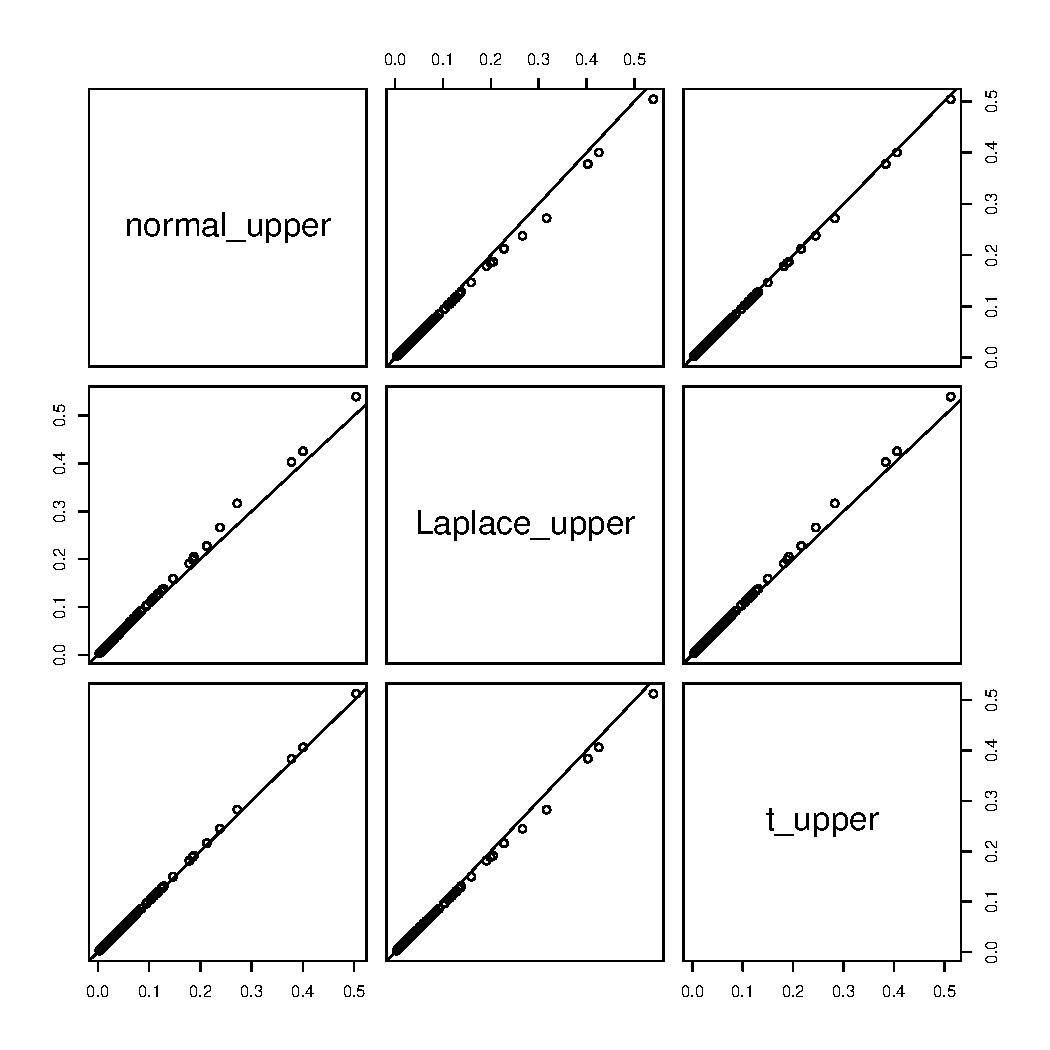
\includegraphics[scale = 0.4]{upper}
\end{minipage} \begin{minipage}{.45\textwidth}
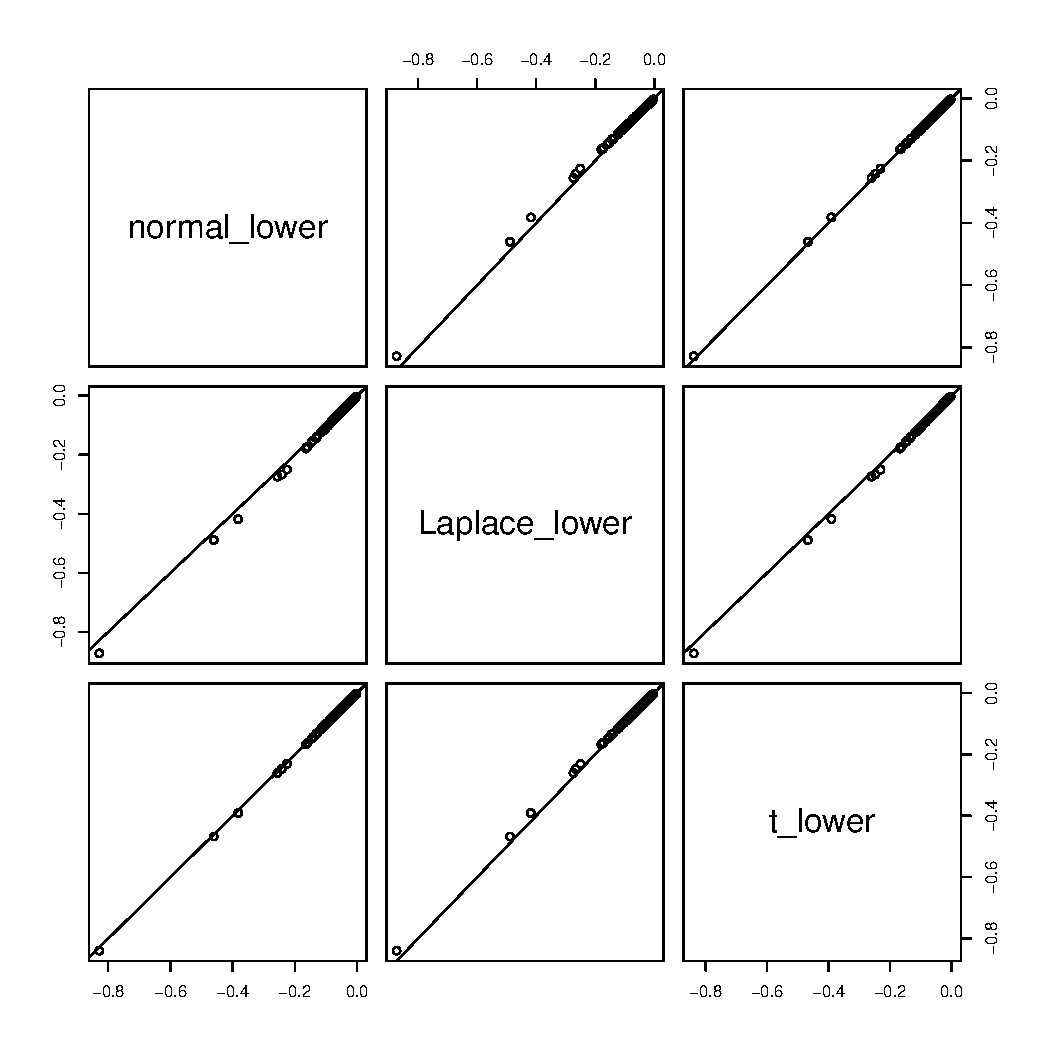
\includegraphics[scale = 0.4]{lower}
\end{minipage}

I suspect that the poor coverage reflects not a bug in the code, but rather a lack of fit quality in our model. From the figures in paper 3, coverage is on par with other models whenever

\begin{enumerate}
\item the true $\beta_{g4}$ values are generated as in the edgeR and Simple scenarios rather than coming from a normal distribution. 
\item a non-horseshoe distribution is applied to the $\beta_{g4}$'s for analysis.
\item we focus on $\beta_{g\ell}$'s for $\ell \ne 4$.
\end{enumerate}

In addition, convergence using the horseshoe was excellent for non-normal simulations and worse for normal ones. On the real data, no Gelman factors exceeded 1.1, not even the ones for the $\epsilon_{gn}$'s. The same was true for the non-normal simulations in Simulation Study 2 except the edgeR scenario with $N = 32$, where $\beta_{6411, 3}$ and $\beta_{6411, 1}$ had Gelman factors of around 1.28. For the normal simulations, however, usually 10-20 parameters had high Gelman factors, almost always including $\sigma_4^2$ ($\widehat{R} \approx 1.5$). 

\end{flushleft}
%\newpage 
%\bibliographystyle{plain} 
%\bibliography{}
\end{document}